% Created by tikzDevice version 0.12.3.1 on 2022-09-02 10:44:49
% !TEX encoding = UTF-8 Unicode
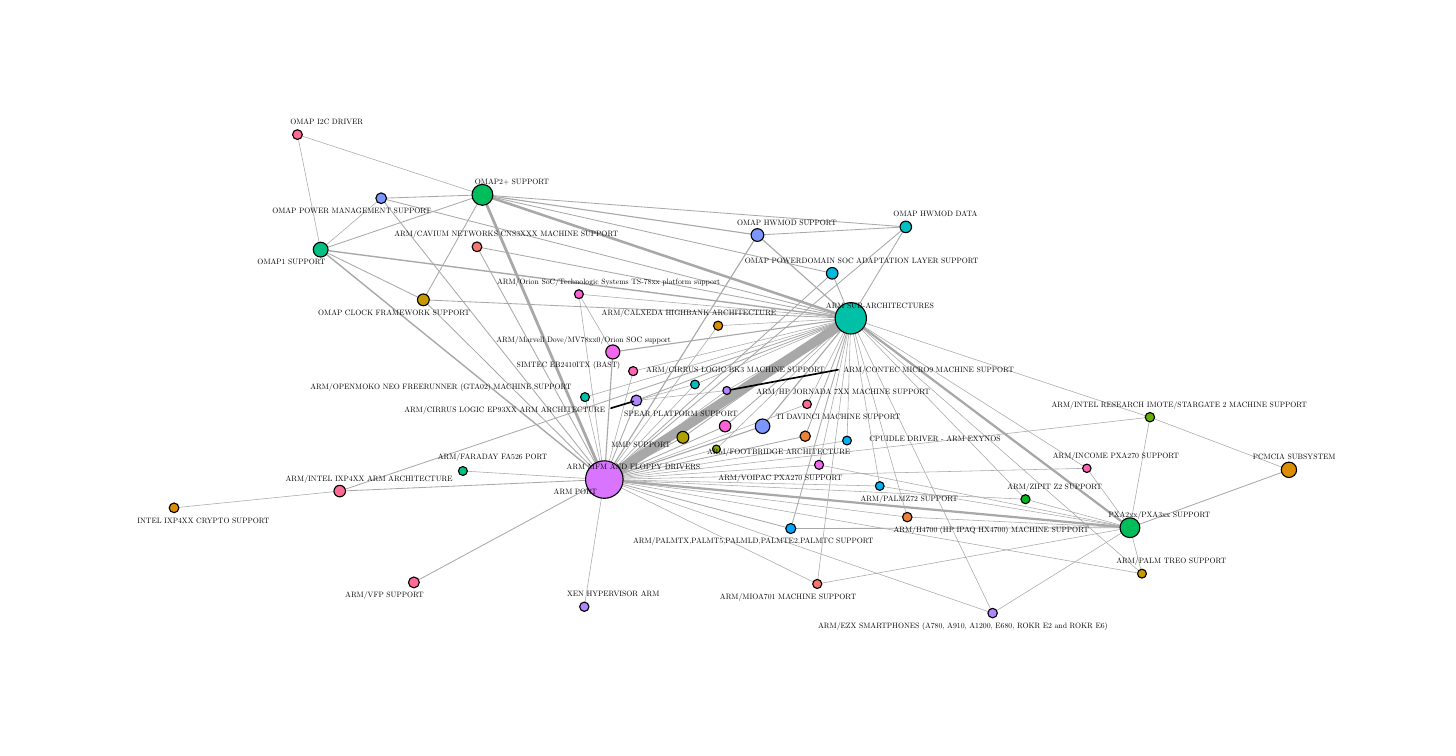
\begin{tikzpicture}[x=1pt,y=1pt]
\definecolor{fillColor}{RGB}{255,255,255}
\path[use as bounding box,fill=fillColor,fill opacity=0.00] (0,0) rectangle (505.89,252.94);
\begin{scope}
\path[clip] (  0.00,  0.00) rectangle (505.89,252.94);
\definecolor{fillColor}{RGB}{255,255,255}

\path[fill=fillColor] (  0.00,  0.00) rectangle (505.89,252.94);
\end{scope}
\begin{scope}
\path[clip] ( 32.75, 32.75) rectangle (475.89,222.94);
\definecolor{drawColor}{gray}{0.66}

\path[draw=drawColor,line width= 0.2pt,line join=round] (248.86,100.68) -- (208.37, 89.65);

\path[draw=drawColor,line width= 0.2pt,line join=round] (248.86,100.68) -- (297.43,147.91);

\path[draw=drawColor,line width= 3.4pt,line join=round] (208.37, 89.65) -- (297.43,147.91);

\path[draw=drawColor,line width= 0.2pt,line join=round] (208.37, 89.65) -- (249.48,145.24);

\path[draw=drawColor,line width= 0.3pt,line join=round] (208.37, 89.65) -- (162.35,173.75);

\path[draw=drawColor,line width= 0.2pt,line join=round] (208.37, 89.65) -- (241.12,124.03);

\path[draw=drawColor,line width= 0.3pt,line join=round] (208.37, 89.65) -- (219.95,118.22);

\path[draw=drawColor,line width= 0.2pt,line join=round] (208.37, 89.65) -- (252.63,121.83);

\path[draw=drawColor,line width= 0.2pt,line join=round] (208.37, 89.65) -- (348.68, 41.40);

\path[draw=drawColor,line width= 0.2pt,line join=round] (208.37, 89.65) -- (157.27, 92.74);

\path[draw=drawColor,line width= 0.3pt,line join=round] (208.37, 89.65) -- (280.96,105.32);

\path[draw=drawColor,line width= 0.2pt,line join=round] (208.37, 89.65) -- (317.84, 76.08);

\path[draw=drawColor,line width= 0.2pt,line join=round] (208.37, 89.65) -- (281.62,116.87);

\path[draw=drawColor,line width= 0.2pt,line join=round] (208.37, 89.65) -- (382.72, 93.72);

\path[draw=drawColor,line width= 0.3pt,line join=round] (208.37, 89.65) -- (112.76, 85.48);

\path[draw=drawColor,line width= 0.2pt,line join=round] (208.37, 89.65) -- (405.52,112.18);

\path[draw=drawColor,line width= 0.2pt,line join=round] (208.37, 89.65) -- (285.31, 51.93);

\path[draw=drawColor,line width= 0.4pt,line join=round] (208.37, 89.65) -- (211.43,135.76);

\path[draw=drawColor,line width= 0.2pt,line join=round] (208.37, 89.65) -- (201.39,119.44);

\path[draw=drawColor,line width= 0.2pt,line join=round] (208.37, 89.65) -- (199.19,156.64);

\path[draw=drawColor,line width= 0.2pt,line join=round] (208.37, 89.65) -- (402.65, 55.65);

\path[draw=drawColor,line width= 0.3pt,line join=round] (208.37, 89.65) -- (275.74, 71.94);

\path[draw=drawColor,line width= 0.2pt,line join=round] (208.37, 89.65) -- (307.90, 87.32);

\path[draw=drawColor,line width= 0.3pt,line join=round] (208.37, 89.65) -- (139.56, 52.48);

\path[draw=drawColor,line width= 0.2pt,line join=round] (208.37, 89.65) -- (285.97, 94.97);

\path[draw=drawColor,line width= 0.2pt,line join=round] (208.37, 89.65) -- (360.55, 82.55);

\path[draw=drawColor,line width= 0.2pt,line join=round] (208.37, 89.65) -- (296.06,103.74);

\path[draw=drawColor,line width= 0.3pt,line join=round] (208.37, 89.65) -- (236.78,104.91);

\path[draw=drawColor,line width= 0.3pt,line join=round] (208.37, 89.65) -- (142.98,154.59);

\path[draw=drawColor,line width= 0.3pt,line join=round] (208.37, 89.65) -- (317.31,180.95);

\path[draw=drawColor,line width= 0.4pt,line join=round] (208.37, 89.65) -- (263.69,178.01);

\path[draw=drawColor,line width= 0.3pt,line join=round] (208.37, 89.65) -- (127.74,191.30);

\path[draw=drawColor,line width= 0.3pt,line join=round] (208.37, 89.65) -- (290.72,164.18);

\path[draw=drawColor,line width= 0.5pt,line join=round] (208.37, 89.65) -- (105.87,172.72);

\path[draw=drawColor,line width= 1.0pt,line join=round] (208.37, 89.65) -- (164.33,192.53);

\path[draw=drawColor,line width= 0.8pt,line join=round] (208.37, 89.65) -- (398.30, 72.25);

\path[draw=drawColor,line width= 0.2pt,line join=round] (208.37, 89.65) -- (218.79,128.82);

\path[draw=drawColor,line width= 0.3pt,line join=round] (208.37, 89.65) -- (252.02,108.96);

\path[draw=drawColor,line width= 0.4pt,line join=round] (208.37, 89.65) -- (265.55,108.91);

\path[draw=drawColor,line width= 0.2pt,line join=round] (208.37, 89.65) -- (201.14, 43.69);

\path[draw=drawColor,line width= 0.2pt,line join=round] (297.43,147.91) -- (249.48,145.24);

\path[draw=drawColor,line width= 0.3pt,line join=round] (297.43,147.91) -- (162.35,173.75);

\path[draw=drawColor,line width= 0.2pt,line join=round] (297.43,147.91) -- (241.12,124.03);

\path[draw=drawColor,line width= 0.3pt,line join=round] (297.43,147.91) -- (219.95,118.22);

\path[draw=drawColor,line width= 0.2pt,line join=round] (297.43,147.91) -- (252.63,121.83);

\path[draw=drawColor,line width= 0.2pt,line join=round] (297.43,147.91) -- (348.68, 41.40);

\path[draw=drawColor,line width= 0.3pt,line join=round] (297.43,147.91) -- (280.96,105.32);

\path[draw=drawColor,line width= 0.2pt,line join=round] (297.43,147.91) -- (317.84, 76.08);

\path[draw=drawColor,line width= 0.2pt,line join=round] (297.43,147.91) -- (281.62,116.87);

\path[draw=drawColor,line width= 0.2pt,line join=round] (297.43,147.91) -- (382.72, 93.72);

\path[draw=drawColor,line width= 0.3pt,line join=round] (297.43,147.91) -- (112.76, 85.48);

\path[draw=drawColor,line width= 0.2pt,line join=round] (297.43,147.91) -- (405.52,112.18);

\path[draw=drawColor,line width= 0.2pt,line join=round] (297.43,147.91) -- (285.31, 51.93);

\path[draw=drawColor,line width= 0.4pt,line join=round] (297.43,147.91) -- (211.43,135.76);

\path[draw=drawColor,line width= 0.2pt,line join=round] (297.43,147.91) -- (201.39,119.44);

\path[draw=drawColor,line width= 0.2pt,line join=round] (297.43,147.91) -- (199.19,156.64);

\path[draw=drawColor,line width= 0.2pt,line join=round] (297.43,147.91) -- (402.65, 55.65);

\path[draw=drawColor,line width= 0.3pt,line join=round] (297.43,147.91) -- (275.74, 71.94);

\path[draw=drawColor,line width= 0.2pt,line join=round] (297.43,147.91) -- (307.90, 87.32);

\path[draw=drawColor,line width= 0.2pt,line join=round] (297.43,147.91) -- (285.97, 94.97);

\path[draw=drawColor,line width= 0.2pt,line join=round] (297.43,147.91) -- (360.55, 82.55);

\path[draw=drawColor,line width= 0.2pt,line join=round] (297.43,147.91) -- (296.06,103.74);

\path[draw=drawColor,line width= 0.3pt,line join=round] (297.43,147.91) -- (236.78,104.91);

\path[draw=drawColor,line width= 0.3pt,line join=round] (297.43,147.91) -- (142.98,154.59);

\path[draw=drawColor,line width= 0.3pt,line join=round] (297.43,147.91) -- (317.31,180.95);

\path[draw=drawColor,line width= 0.4pt,line join=round] (297.43,147.91) -- (263.69,178.01);

\path[draw=drawColor,line width= 0.3pt,line join=round] (297.43,147.91) -- (127.74,191.30);

\path[draw=drawColor,line width= 0.3pt,line join=round] (297.43,147.91) -- (290.72,164.18);

\path[draw=drawColor,line width= 0.5pt,line join=round] (297.43,147.91) -- (105.87,172.72);

\path[draw=drawColor,line width= 0.9pt,line join=round] (297.43,147.91) -- (164.33,192.53);

\path[draw=drawColor,line width= 0.8pt,line join=round] (297.43,147.91) -- (398.30, 72.25);

\path[draw=drawColor,line width= 0.2pt,line join=round] (297.43,147.91) -- (218.79,128.82);

\path[draw=drawColor,line width= 0.3pt,line join=round] (297.43,147.91) -- (252.02,108.96);

\path[draw=drawColor,line width= 0.4pt,line join=round] (297.43,147.91) -- (265.55,108.91);

\path[draw=drawColor,line width= 0.2pt,line join=round] (241.12,124.03) -- (219.95,118.22);

\path[draw=drawColor,line width= 0.2pt,line join=round] (219.95,118.22) -- (252.63,121.83);

\path[draw=drawColor,line width= 0.2pt,line join=round] (348.68, 41.40) -- (398.30, 72.25);

\path[draw=drawColor,line width= 0.2pt,line join=round] (317.84, 76.08) -- (398.30, 72.25);

\path[draw=drawColor,line width= 0.2pt,line join=round] (382.72, 93.72) -- (398.30, 72.25);

\path[draw=drawColor,line width= 0.2pt,line join=round] (112.76, 85.48) -- ( 52.89, 79.43);

\path[draw=drawColor,line width= 0.2pt,line join=round] (405.52,112.18) -- (455.75, 93.17);

\path[draw=drawColor,line width= 0.2pt,line join=round] (405.52,112.18) -- (398.30, 72.25);

\path[draw=drawColor,line width= 0.2pt,line join=round] (285.31, 51.93) -- (398.30, 72.25);

\path[draw=drawColor,line width= 0.2pt,line join=round] (211.43,135.76) -- (199.19,156.64);

\path[draw=drawColor,line width= 0.2pt,line join=round] (402.65, 55.65) -- (398.30, 72.25);

\path[draw=drawColor,line width= 0.3pt,line join=round] (275.74, 71.94) -- (398.30, 72.25);

\path[draw=drawColor,line width= 0.2pt,line join=round] (307.90, 87.32) -- (398.30, 72.25);

\path[draw=drawColor,line width= 0.2pt,line join=round] (285.97, 94.97) -- (398.30, 72.25);

\path[draw=drawColor,line width= 0.2pt,line join=round] (360.55, 82.55) -- (398.30, 72.25);

\path[draw=drawColor,line width= 0.3pt,line join=round] (142.98,154.59) -- (105.87,172.72);

\path[draw=drawColor,line width= 0.3pt,line join=round] (142.98,154.59) -- (164.33,192.53);

\path[draw=drawColor,line width= 0.3pt,line join=round] (317.31,180.95) -- (263.69,178.01);

\path[draw=drawColor,line width= 0.3pt,line join=round] (317.31,180.95) -- (164.33,192.53);

\path[draw=drawColor,line width= 0.4pt,line join=round] (263.69,178.01) -- (164.33,192.53);

\path[draw=drawColor,line width= 0.2pt,line join=round] ( 97.48,214.30) -- (105.87,172.72);

\path[draw=drawColor,line width= 0.2pt,line join=round] ( 97.48,214.30) -- (164.33,192.53);

\path[draw=drawColor,line width= 0.2pt,line join=round] (127.74,191.30) -- (105.87,172.72);

\path[draw=drawColor,line width= 0.3pt,line join=round] (127.74,191.30) -- (164.33,192.53);

\path[draw=drawColor,line width= 0.3pt,line join=round] (290.72,164.18) -- (164.33,192.53);

\path[draw=drawColor,line width= 0.3pt,line join=round] (105.87,172.72) -- (164.33,192.53);

\path[draw=drawColor,line width= 0.3pt,line join=round] (455.75, 93.17) -- (398.30, 72.25);
\definecolor{drawColor}{RGB}{0,0,0}
\definecolor{fillColor}{RGB}{143,170,0}

\path[draw=drawColor,line width= 0.4pt,line join=round,line cap=round,fill=fillColor] (248.86,100.68) circle (  1.43);
\definecolor{fillColor}{RGB}{216,116,253}

\path[draw=drawColor,line width= 0.4pt,line join=round,line cap=round,fill=fillColor] (208.37, 89.65) circle (  6.78);
\definecolor{fillColor}{RGB}{0,193,167}

\path[draw=drawColor,line width= 0.4pt,line join=round,line cap=round,fill=fillColor] (297.43,147.91) circle (  5.66);
\definecolor{fillColor}{RGB}{219,142,0}

\path[draw=drawColor,line width= 0.4pt,line join=round,line cap=round,fill=fillColor] (249.48,145.24) circle (  1.66);
\definecolor{fillColor}{RGB}{248,118,109}

\path[draw=drawColor,line width= 0.4pt,line join=round,line cap=round,fill=fillColor] (162.35,173.75) circle (  1.77);
\definecolor{fillColor}{RGB}{0,191,196}

\path[draw=drawColor,line width= 0.4pt,line join=round,line cap=round,fill=fillColor] (241.12,124.03) circle (  1.57);
\definecolor{fillColor}{RGB}{179,133,255}

\path[draw=drawColor,line width= 0.4pt,line join=round,line cap=round,fill=fillColor] (219.95,118.22) circle (  1.96);

\path[draw=drawColor,line width= 0.4pt,line join=round,line cap=round,fill=fillColor] (252.63,121.83) circle (  1.45);

\path[draw=drawColor,line width= 0.4pt,line join=round,line cap=round,fill=fillColor] (348.68, 41.40) circle (  1.71);
\definecolor{fillColor}{RGB}{0,192,133}

\path[draw=drawColor,line width= 0.4pt,line join=round,line cap=round,fill=fillColor] (157.27, 92.74) circle (  1.61);
\definecolor{fillColor}{RGB}{236,130,57}

\path[draw=drawColor,line width= 0.4pt,line join=round,line cap=round,fill=fillColor] (280.96,105.32) circle (  1.88);

\path[draw=drawColor,line width= 0.4pt,line join=round,line cap=round,fill=fillColor] (317.84, 76.08) circle (  1.71);
\definecolor{fillColor}{RGB}{255,107,148}

\path[draw=drawColor,line width= 0.4pt,line join=round,line cap=round,fill=fillColor] (281.62,116.87) circle (  1.57);
\definecolor{fillColor}{RGB}{255,99,182}

\path[draw=drawColor,line width= 0.4pt,line join=round,line cap=round,fill=fillColor] (382.72, 93.72) circle (  1.52);
\definecolor{fillColor}{RGB}{255,107,148}

\path[draw=drawColor,line width= 0.4pt,line join=round,line cap=round,fill=fillColor] (112.76, 85.48) circle (  2.08);
\definecolor{fillColor}{RGB}{100,178,0}

\path[draw=drawColor,line width= 0.4pt,line join=round,line cap=round,fill=fillColor] (405.52,112.18) circle (  1.70);
\definecolor{fillColor}{RGB}{248,118,109}

\path[draw=drawColor,line width= 0.4pt,line join=round,line cap=round,fill=fillColor] (285.31, 51.93) circle (  1.64);
\definecolor{fillColor}{RGB}{239,103,235}

\path[draw=drawColor,line width= 0.4pt,line join=round,line cap=round,fill=fillColor] (211.43,135.76) circle (  2.54);
\definecolor{fillColor}{RGB}{0,193,167}

\path[draw=drawColor,line width= 0.4pt,line join=round,line cap=round,fill=fillColor] (201.39,119.44) circle (  1.61);
\definecolor{fillColor}{RGB}{253,97,211}

\path[draw=drawColor,line width= 0.4pt,line join=round,line cap=round,fill=fillColor] (199.19,156.64) circle (  1.61);
\definecolor{fillColor}{RGB}{199,152,0}

\path[draw=drawColor,line width= 0.4pt,line join=round,line cap=round,fill=fillColor] (402.65, 55.65) circle (  1.61);
\definecolor{fillColor}{RGB}{0,166,255}

\path[draw=drawColor,line width= 0.4pt,line join=round,line cap=round,fill=fillColor] (275.74, 71.94) circle (  1.82);
\definecolor{fillColor}{RGB}{0,178,243}

\path[draw=drawColor,line width= 0.4pt,line join=round,line cap=round,fill=fillColor] (307.90, 87.32) circle (  1.57);
\definecolor{fillColor}{RGB}{255,107,148}

\path[draw=drawColor,line width= 0.4pt,line join=round,line cap=round,fill=fillColor] (139.56, 52.48) circle (  1.96);
\definecolor{fillColor}{RGB}{239,103,235}

\path[draw=drawColor,line width= 0.4pt,line join=round,line cap=round,fill=fillColor] (285.97, 94.97) circle (  1.64);
\definecolor{fillColor}{RGB}{0,184,27}

\path[draw=drawColor,line width= 0.4pt,line join=round,line cap=round,fill=fillColor] (360.55, 82.55) circle (  1.64);
\definecolor{fillColor}{RGB}{0,178,243}

\path[draw=drawColor,line width= 0.4pt,line join=round,line cap=round,fill=fillColor] (296.06,103.74) circle (  1.59);
\definecolor{fillColor}{RGB}{219,142,0}

\path[draw=drawColor,line width= 0.4pt,line join=round,line cap=round,fill=fillColor] ( 52.89, 79.43) circle (  1.75);
\definecolor{fillColor}{RGB}{174,162,0}

\path[draw=drawColor,line width= 0.4pt,line join=round,line cap=round,fill=fillColor] (236.78,104.91) circle (  2.15);
\definecolor{fillColor}{RGB}{199,152,0}

\path[draw=drawColor,line width= 0.4pt,line join=round,line cap=round,fill=fillColor] (142.98,154.59) circle (  2.13);
\definecolor{fillColor}{RGB}{0,191,196}

\path[draw=drawColor,line width= 0.4pt,line join=round,line cap=round,fill=fillColor] (317.31,180.95) circle (  2.08);
\definecolor{fillColor}{RGB}{124,150,255}

\path[draw=drawColor,line width= 0.4pt,line join=round,line cap=round,fill=fillColor] (263.69,178.01) circle (  2.30);
\definecolor{fillColor}{RGB}{255,107,148}

\path[draw=drawColor,line width= 0.4pt,line join=round,line cap=round,fill=fillColor] ( 97.48,214.30) circle (  1.76);
\definecolor{fillColor}{RGB}{124,150,255}

\path[draw=drawColor,line width= 0.4pt,line join=round,line cap=round,fill=fillColor] (127.74,191.30) circle (  1.93);
\definecolor{fillColor}{RGB}{0,186,222}

\path[draw=drawColor,line width= 0.4pt,line join=round,line cap=round,fill=fillColor] (290.72,164.18) circle (  2.09);
\definecolor{fillColor}{RGB}{0,192,133}

\path[draw=drawColor,line width= 0.4pt,line join=round,line cap=round,fill=fillColor] (105.87,172.72) circle (  2.67);
\definecolor{fillColor}{RGB}{0,189,92}

\path[draw=drawColor,line width= 0.4pt,line join=round,line cap=round,fill=fillColor] (164.33,192.53) circle (  3.77);
\definecolor{fillColor}{RGB}{219,142,0}

\path[draw=drawColor,line width= 0.4pt,line join=round,line cap=round,fill=fillColor] (455.75, 93.17) circle (  2.77);
\definecolor{fillColor}{RGB}{0,189,92}

\path[draw=drawColor,line width= 0.4pt,line join=round,line cap=round,fill=fillColor] (398.30, 72.25) circle (  3.58);
\definecolor{fillColor}{RGB}{255,99,182}

\path[draw=drawColor,line width= 0.4pt,line join=round,line cap=round,fill=fillColor] (218.79,128.82) circle (  1.65);
\definecolor{fillColor}{RGB}{253,97,211}

\path[draw=drawColor,line width= 0.4pt,line join=round,line cap=round,fill=fillColor] (252.02,108.96) circle (  2.06);
\definecolor{fillColor}{RGB}{124,150,255}

\path[draw=drawColor,line width= 0.4pt,line join=round,line cap=round,fill=fillColor] (265.55,108.91) circle (  2.63);
\definecolor{fillColor}{RGB}{179,133,255}

\path[draw=drawColor,line width= 0.4pt,line join=round,line cap=round,fill=fillColor] (201.14, 43.69) circle (  1.68);

\path[draw=drawColor,line width= 0.6pt,line join=round,line cap=round] (210.76,115.44) -- (218.91,117.91);

\path[draw=drawColor,line width= 0.6pt,line join=round,line cap=round] (292.80,129.32) -- (253.79,122.05);

\node[text=drawColor,anchor=base,inner sep=0pt, outer sep=0pt, scale=  0.28] at (218.92, 93.21) {ARM MFM AND FLOPPY DRIVERS};

\node[text=drawColor,anchor=base,inner sep=0pt, outer sep=0pt, scale=  0.28] at (197.89, 84.14) {ARM PORT};

\node[text=drawColor,anchor=base,inner sep=0pt, outer sep=0pt, scale=  0.28] at (307.98,151.46) {ARM SUB-ARCHITECTURES};

\node[text=drawColor,anchor=base,inner sep=0pt, outer sep=0pt, scale=  0.28] at (238.97,148.79) {ARM/CALXEDA HIGHBANK ARCHITECTURE};

\node[text=drawColor,anchor=base,inner sep=0pt, outer sep=0pt, scale=  0.28] at (172.95,177.33) {ARM/CAVIUM NETWORKS CNS3XXX MACHINE SUPPORT};

\node[text=drawColor,anchor=base,inner sep=0pt, outer sep=0pt, scale=  0.28] at (255.78,128.49) {ARM/CIRRUS LOGIC BK3 MACHINE SUPPORT};

\node[text=drawColor,anchor=base,inner sep=0pt, outer sep=0pt, scale=  0.28] at (172.40,113.92) {ARM/CIRRUS LOGIC EP93XX ARM ARCHITECTURE};

\node[text=drawColor,anchor=base,inner sep=0pt, outer sep=0pt, scale=  0.28] at (325.58,128.45) {ARM/CONTEC MICRO9 MACHINE SUPPORT};

\node[text=drawColor,anchor=base,inner sep=0pt, outer sep=0pt, scale=  0.28] at (337.95, 35.85) {ARM/EZX SMARTPHONES (A780, A910, A1200, E680, ROKR E2 and ROKR E6)};

\node[text=drawColor,anchor=base,inner sep=0pt, outer sep=0pt, scale=  0.28] at (167.99, 97.02) {ARM/FARADAY FA526 PORT};

\node[text=drawColor,anchor=base,inner sep=0pt, outer sep=0pt, scale=  0.28] at (271.37, 98.54) {ARM/FOOTBRIDGE ARCHITECTURE};

\node[text=drawColor,anchor=base,inner sep=0pt, outer sep=0pt, scale=  0.28] at (348.19, 70.56) {ARM/H4700 (HP IPAQ HX4700) MACHINE SUPPORT};

\node[text=drawColor,anchor=base,inner sep=0pt, outer sep=0pt, scale=  0.28] at (294.71,120.44) {ARM/HP JORNADA 7XX MACHINE SUPPORT};

\node[text=drawColor,anchor=base,inner sep=0pt, outer sep=0pt, scale=  0.28] at (393.26, 97.27) {ARM/INCOME PXA270 SUPPORT};

\node[text=drawColor,anchor=base,inner sep=0pt, outer sep=0pt, scale=  0.28] at (123.39, 89.05) {ARM/INTEL IXP4XX ARM ARCHITECTURE};

\node[text=drawColor,anchor=base,inner sep=0pt, outer sep=0pt, scale=  0.28] at (416.14,115.73) {ARM/INTEL RESEARCH IMOTE/STARGATE 2 MACHINE SUPPORT};

\node[text=drawColor,anchor=base,inner sep=0pt, outer sep=0pt, scale=  0.28] at (274.76, 46.41) {ARM/MIOA701 MACHINE SUPPORT};

\node[text=drawColor,anchor=base,inner sep=0pt, outer sep=0pt, scale=  0.28] at (200.90,139.31) {ARM/Marvell Dove/MV78xx0/Orion SOC support};

\node[text=drawColor,anchor=base,inner sep=0pt, outer sep=0pt, scale=  0.28] at (149.31,122.23) {ARM/OPENMOKO NEO FREERUNNER (GTA02) MACHINE SUPPORT};

\node[text=drawColor,anchor=base,inner sep=0pt, outer sep=0pt, scale=  0.28] at (209.91,160.24) {ARM/Orion SoC/Technologic Systems TS-78xx platform support};

\node[text=drawColor,anchor=base,inner sep=0pt, outer sep=0pt, scale=  0.28] at (413.25, 59.24) {ARM/PALM TREO SUPPORT};

\node[text=drawColor,anchor=base,inner sep=0pt, outer sep=0pt, scale=  0.28] at (262.20, 66.43) {ARM/PALMTX,PALMT5,PALMLD,PALMTE2,PALMTC SUPPORT};

\node[text=drawColor,anchor=base,inner sep=0pt, outer sep=0pt, scale=  0.28] at (318.57, 81.80) {ARM/PALMZ72 SUPPORT};

\node[text=drawColor,anchor=base,inner sep=0pt, outer sep=0pt, scale=  0.28] at (128.94, 46.97) {ARM/VFP SUPPORT};

\node[text=drawColor,anchor=base,inner sep=0pt, outer sep=0pt, scale=  0.28] at (271.98, 89.44) {ARM/VOIPAC PXA270 SUPPORT};

\node[text=drawColor,anchor=base,inner sep=0pt, outer sep=0pt, scale=  0.28] at (371.10, 86.13) {ARM/ZIPIT Z2 SUPPORT};

\node[text=drawColor,anchor=base,inner sep=0pt, outer sep=0pt, scale=  0.28] at (327.85,103.34) {CPUIDLE DRIVER - ARM EXYNOS};

\node[text=drawColor,anchor=base,inner sep=0pt, outer sep=0pt, scale=  0.28] at ( 63.50, 73.87) {INTEL IXP4XX CRYPTO SUPPORT};

\node[text=drawColor,anchor=base,inner sep=0pt, outer sep=0pt, scale=  0.28] at (221.63,101.21) {MMP SUPPORT};

\node[text=drawColor,anchor=base,inner sep=0pt, outer sep=0pt, scale=  0.28] at (132.41,149.05) {OMAP CLOCK FRAMEWORK SUPPORT};

\node[text=drawColor,anchor=base,inner sep=0pt, outer sep=0pt, scale=  0.28] at (328.01,184.53) {OMAP HWMOD DATA};

\node[text=drawColor,anchor=base,inner sep=0pt, outer sep=0pt, scale=  0.28] at (274.32,181.60) {OMAP HWMOD SUPPORT};

\node[text=drawColor,anchor=base,inner sep=0pt, outer sep=0pt, scale=  0.28] at (108.06,217.85) {OMAP I2C DRIVER};

\node[text=drawColor,anchor=base,inner sep=0pt, outer sep=0pt, scale=  0.28] at (117.07,185.75) {OMAP POWER MANAGEMENT SUPPORT};

\node[text=drawColor,anchor=base,inner sep=0pt, outer sep=0pt, scale=  0.28] at (301.36,167.74) {OMAP POWERDOMAIN SOC ADAPTATION LAYER SUPPORT};

\node[text=drawColor,anchor=base,inner sep=0pt, outer sep=0pt, scale=  0.28] at ( 95.33,167.19) {OMAP1 SUPPORT};

\node[text=drawColor,anchor=base,inner sep=0pt, outer sep=0pt, scale=  0.28] at (175.00,196.15) {OMAP2+ SUPPORT};

\node[text=drawColor,anchor=base,inner sep=0pt, outer sep=0pt, scale=  0.28] at (457.66, 96.73) {PCMCIA SUBSYSTEM};

\node[text=drawColor,anchor=base,inner sep=0pt, outer sep=0pt, scale=  0.28] at (408.95, 75.82) {PXA2xx/PXA3xx SUPPORT};

\node[text=drawColor,anchor=base,inner sep=0pt, outer sep=0pt, scale=  0.28] at (195.42,130.23) {SIMTEC EB2410ITX (BAST)};

\node[text=drawColor,anchor=base,inner sep=0pt, outer sep=0pt, scale=  0.28] at (236.06,112.51) {SPEAR PLATFORM SUPPORT};

\node[text=drawColor,anchor=base,inner sep=0pt, outer sep=0pt, scale=  0.28] at (292.82,111.31) {TI DAVINCI MACHINE SUPPORT};

\node[text=drawColor,anchor=base,inner sep=0pt, outer sep=0pt, scale=  0.28] at (211.59, 47.23) {XEN HYPERVISOR ARM};
\end{scope}
\end{tikzpicture}
